\subsection*{Ejercicio 4}

Para crear un vector ordenado he usado la siguiente modificación:

\begin{verbatim}
  v[0] = 0;
  for (int i=1; i<tam; i++){  // Recorrer vector
    v[i] = v[i-1] + rand() % 50;    // Generar aleatorio [0,vmax[
  }
\end{verbatim}

y para crear un vector decreciente:

\begin{verbatim}
  v[0] = vmax;
  for (int i=1; i<tam; i++){  // Recorrer vector
    v[i] = v[i-1] - rand() % 100;    // Generar aleatorio [0,vmax[
  }
\end{verbatim}

El resultado ha sido el siguiente:

\begin{figure}[H]
  \caption{Comparación de modificaciones en el algoritmo bubble sort}
  \centering
    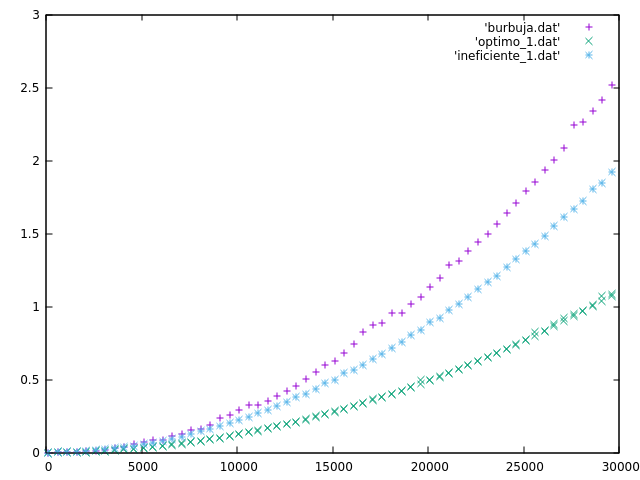
\includegraphics[width=0.8\textwidth]{final.png}
\end{figure}